% ****** Start of file MolecularSpinFlipLoss.tex ******
%
%
%

\documentclass[%
 reprint,
%superscriptaddress,
groupedaddress,
%unsortedaddress,
%runinaddress,
%frontmatterverbose, 
%preprint,
%showpacs,preprintnumbers,
%nofootinbib,
%nobibnotes,
%bibnotes,
 amsmath,amssymb,
 aps,
prl,
%pra,
%prb,
%rmp,
%prstab,
%prstper,
%floatfix,
]{revtex4-1}

\usepackage{graphicx}% Include figure files
\usepackage{dcolumn}% Align table columns on decimal point
\usepackage{bm}% bold math
\usepackage[hidelinks]{hyperref}% add hypertext capabilities
%\usepackage[mathlines]{lineno}% Enable numbering of text and display math
%\linenumbers\relax % Commence numbering lines

%\usepackage[showframe,%Uncomment any one of the following lines to test 
%%scale=0.7, marginratio={1:1, 2:3}, ignoreall,% default settings
%%text={7in,10in},centering,
%%margin=1.5in,
%%total={6.5in,8.75in}, top=1.2in, left=0.9in, includefoot,
%%height=10in,a5paper,hmargin={3cm,0.8in},
%]{geometry}

\newcommand{\epb}{$E\!\perp\!B$}
\newcommand{\epbm}{E\!\perp\!B}

\begin{document}

%\preprint{APS/123-QED}

\title{A Dual Quadrupole Trap for Molecular Spin-Flip Loss}%

\author{David Reens}
\altaffiliation{dave.reens@colorado.edu}%
\author{Hao Wu}
\author{Tim Langen}%
\altaffiliation{Present Address: 5. Physikalisches Institut and Center for Integrated Quantum Science and Technology (IQST), Universit\"at Stuttgart, Pfaffenwaldring 57, 70569 Stuttgart, Germany}
\author{Jun Ye}
\affiliation{%
JILA, National Institute of Standards and Technology
and the University of Colorado \\ Department of Physics, University
of Colorado, Boulder, Colorado 80309-0440, USA
}%

\date{\today}% It is always \today, today,


%%%%%%%%%%%%%%%%%%%%%
%ABSTRACT
%%%%%%%%%%%%%%%%%%%%%
\begin{abstract}
A new electromagnetic trap geometry allows full tuning of complex molecular spin-dynamics in crossed electric and magnetic fields. If not tuned properly, these dynamics lead to spin-flip loss that afflicts a wide set of candidate molecules. The spin-flip loss can be significant even above $100\text{ mK}$ and increases with $1/T$, so it's removal represents a critical step toward ultracold molecules. The trapping geometry features a $0.5 \text{ K}$ trap depth and $5 \text{ T/cm}$ trap strength, and allows spin-dynamics to be tuned with a weak external bias coil. Spin-flip loss is tuned in a $170 \text{ mK}$ sample of OH molecules from over $200 \text{ s}^{-1} $ to below the vacuum limited lifetime of $2 \text{ s}^{-1}$.
\end{abstract}


\maketitle


%%%%%%%%%%%%%%%%%%%%%%%%%%%%%%%%%
%
%     III   NNN   TTT   RRR   OOO   DDD   UUU   CCC   TTT   III   OOO   NNN
%     III   NNN   TTT   RRR   OOO   DDD   UUU   CCC   TTT   III   OOO   NNN
%     III   NNN   TTT   RRR   OOO   DDD   UUU   CCC   TTT   III   OOO   NNN
%
%%%%%%%%%%%%%%%%%%%%%%%%%%%%%%%%%
%\section{Introduction}
The ultracold regime extends toward molecules on many fronts~\cite{Carr2009}. Several bialkali molecules are available~\cite{Ni2008, Takekoshi2014, Park2015} and others are under development. Creative and carefully engineered laser cooling strategies are tackling certain nearly vibrationally diagonal molecules~\cite{Steinecker2016, Barry2014, Hemmerling2016, Hummon2013, Zhelyazkova2014}. A plethora of non-optical cooling strategies have succeeded to greater or lesser extents on other molecules~\cite{Doyle1998,Prehn2016,Bethlem1999,Bochinski2003,Akerman2015}. All of these molecules will require secondary strategies like evaporation or sympathetic cooling to make further gains in phase space density. They also may face a familiar challenge: spin flip loss near the zero of a magnetic trap, but dramatically enhanced for many doubly dipolar molecules due to their internal spin dynamics in mixed electric and magnetic fields. 

The knowledge of spin flips or Majorana hops as an eventual trap lifetime limit predates the very first magnetic trapping of neutrals~\cite{Migdall1985}. Spin flips were directly observed near $10\,\mu\text{K}$ and overcome in the TOP trap~\cite{Petrich1995}, and soon later with a plugged dipole trap~\cite{Davis1995}, famously enabling the first Bose-Einstein condensates. We observe spin-flips in a $170\text{ mK}$ OH sample, four orders of magnitude higher in temperature compared with the atomic case. We observe this and tune it in our new dual magnetic and electric quadrupole trap, but it also applies to our previous geometry~\cite{Sawyer2008}, a 3D permanent magnet quadrupole trap, when homogeneous electric field is applied. We use this simpler geometry, detailed in panels (d) and (e) of fig.~\ref{fig:blocking}, as our starting point to explain the internal spin-dynamics that lead to the spin-flip loss. We then explain our new trapping geometry and how it achieves tunable removal of spin-flip loss. The internal spin-dynamics are applicable to Hund's case A molecules and also to Hund's case B to a lesser extent.%In previous iterations of our OH trapping experiment, and in the most recent described here, we have observed molecular spin-flips at four order higher temperatures in the $45-170\text{ mK}$ range. The loss is connected to the doubly dipolar nature of molecules and thus to their behavior in mixed electric and magnetic fields. Such field mixing arises in any experiment which aims to take advantage of this doubly dipolar nature. The loss varies in 

%The observation was discussed briefly in the appendix of~\cite{Stuhl2013}. 

\begin{figure}[tb]
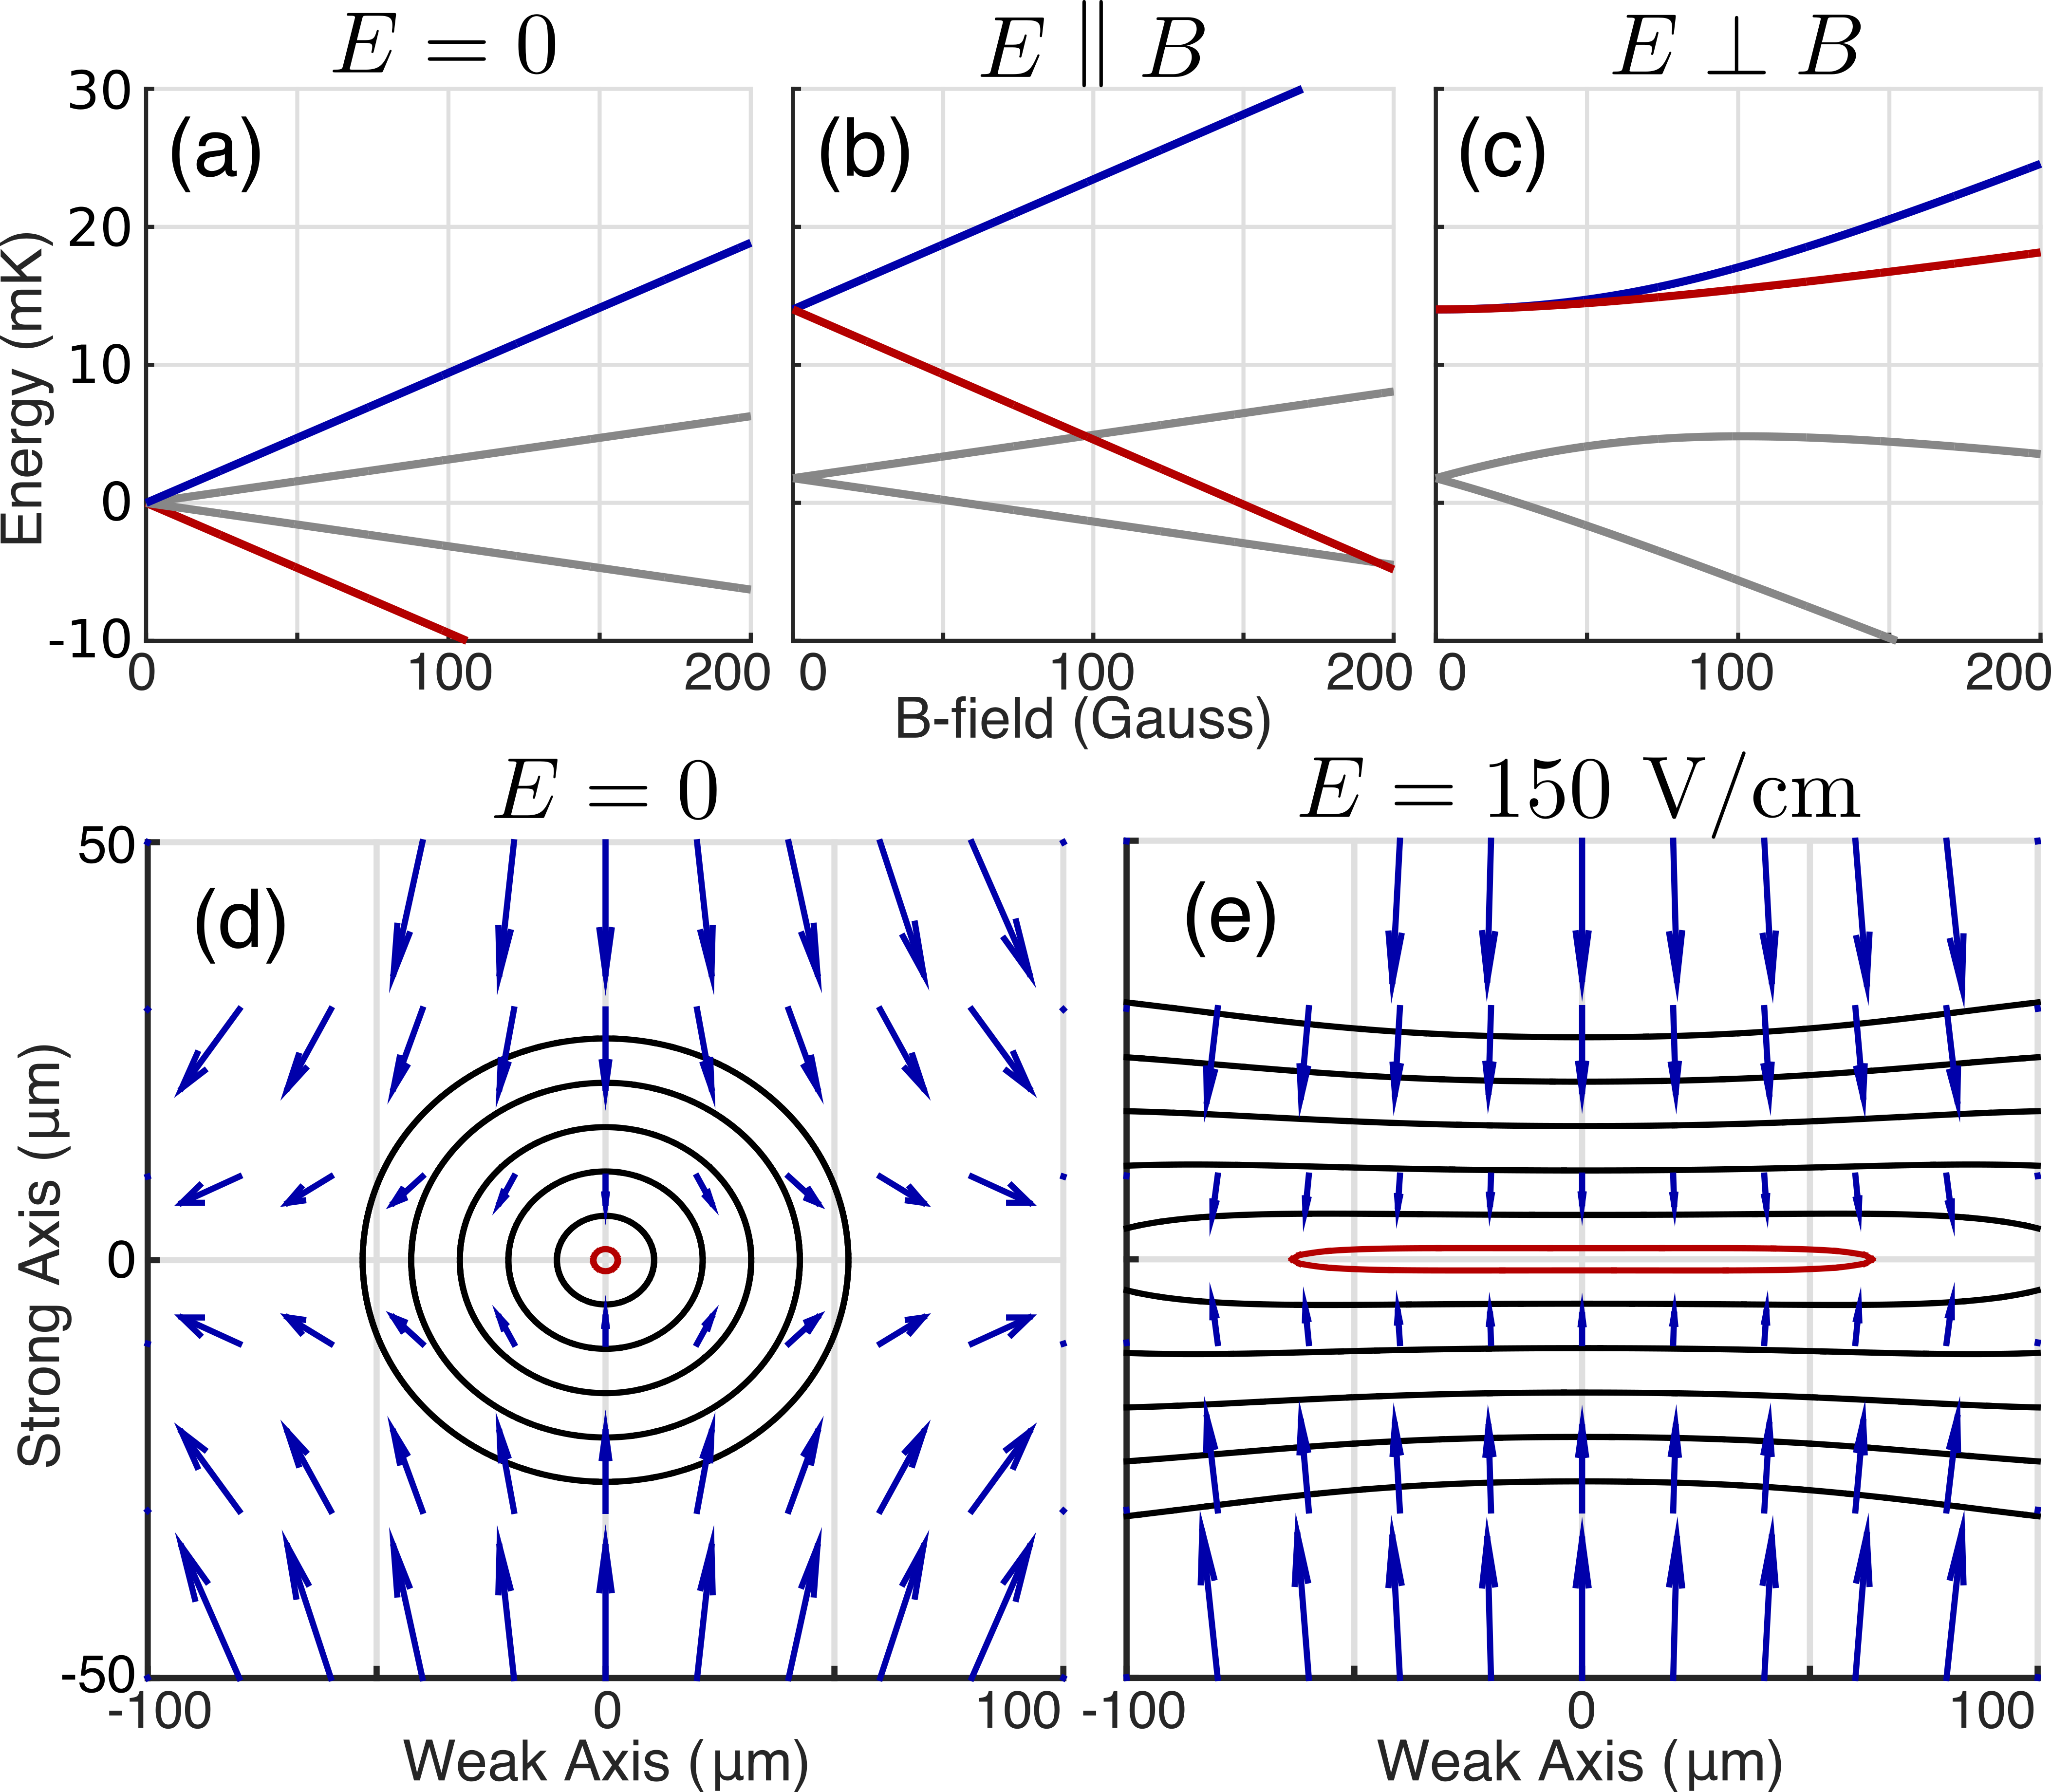
\includegraphics[width=\linewidth]{Blocking/blocking.png}%
\caption{
The blocking effect. (a), four Zeeman split lines in OH's $J=3/2$ ground manifold. A nearly identical set of opposite parity lie $1.7\text{ GHz}$ below. The trapped state (blue) and it's spin-flip partner (red). (b) Zeeman splitting, $E||B$, $E=150\text{V/cm}$. (c) \epb. Note vastly reduced red-blue splitting. See all angles in appendix of~\cite{Stuhl2013}. (d) Energy splitting contours every 2 mK near the zero of our $2\text{ T/cm}$ trap~\cite{Stuhl2012uwave}. B-field arrows in blue. (e) Again with $E=150\text{ V/cm}$. Note drastic widening of lowest contour (red). Vector direction gives the Hund's Case X quantization axis of trapped state, $\mu_BB\pm d_EE$ above (below) the center plane. Vector magnitude gives potential energy relative to trap center.
\label{fig:blocking}}
\end{figure}

%The electric field leads to a significant population decay beyond background gas collisions, initially attributed to collisional tuning. We now realize that the internal spin-dynamics of the molecules also result in these losses, with a magnitude sufficiently comparable so as to preclude deconvolution of any remaining collisional effect.\footnote{The existence of the internal spin-dynamical effect was known and described in the appendix of~\cite{Stuhl2013}, but more thorough recent investigations have demonstrated it to be of larger magnitude.} 

The internal spin-dynamics that lead to this enhanced spin-flip loss are subtle, having eluded three previous investigations. In~\cite{Lara2008} the analogues of atomic spin-flip loss for molecules in mixed fields were investigated, and our focus case, a magnetic quadrupole trap for OH molecules with superposed electric field, was specifically addressed. It was concluded that no significant loss enhancement due to electric field should be evident. While this is true for the approximate $^2\Pi_{1/2}$ Hamiltonian used in that study, it is not true for the actual $^2\Pi_{3/2}$ ground state of OH. Motivated by suggestions of intriguing collisional physics, in~\cite{Stuhl2013} electric field induced collisions were studied. Although an effort was made to deconvolve molecular spin-flip loss, the magnitudes were underestimated.~\footnote{It is unclear how much of a collisional effect described in~\cite{Stuhl2013} remains. This will need to be the subject of further investigation.} Finally, in~\cite{Bohn2013} it was correctly noted that Hund's case A molecules maintain a quantization axis in mixed fields. In fact the states of the molecule align with one of two quantization axes- either the vector sum or the vector difference of the dipole moment weighted electric and magnetic fields. It was asserted that this would maintain quantization near the zero of a quadrupole trap and avoid spin-flip loss. Quantization is maintained, but spin-flip loss is enhanced.

This is actually the crux of the internal spin-dynamics that lead to loss. With only magnetic field, a molecule remains trapped insofar as it adiabatically follows the field direction. Near the trap center, the direction changes most rapidly, enabling loss. When electric field is added, it dominates in the trap center where the magnetic field is weakest. Quantization is maintained but the quantization axis does not rotate with the magnetic field as it needs to. Further away from the trap center the molecule is then magnetically strong field seeking and is lost. The molecule ought to have switched from the vector sum quantization axis to the vector difference quantization axis, so as to remain doubly weak field seeking despite the change in relative orientation of the fields. \footnote{Without the lambda doubling perturbation, which connects the substates of different quantization axes and provides a barrier supportive of remaining in the doubly dipolar substate, a perfectly linear Stark effect molecule would be lost with unit probability anywhere in the orthogonal plane.}%So how could this occur while quantization is maintained? When electric field is added, there are actually two different quantization axes, obtained by either adding or subtracting the dipole moment weighted field vectors. In order to remain trapped a dipolar molecule must remain doubly stretched by the two fields, requiring alignment with either the vector addition or the vector subtraction quantization axis depending on whether the fields point toward or away from one another. In part of the trap fields point in the same direction, but on the other side they point opposite. Thus maintaining quantization axis is actually an impediment to remaining in the well trapped substate- the molecule must hop from one quantization axis to the other in order to remain trapped.

In terms of energies, this manifests as an unusually narrow Zeeman splitting in the region where the relative field orientation changes, i.e. where the fields are orthogonal. In our focus case this occurs in a plane through the trap center, but generally it is always a 2D region since it is a level set of the continuous scalar $\phi = E\cdot B$. In the subset of this plane where $\mu_BB<<d_EE$, the Zeeman effect is not linear but cubic. We call this ``blocking", see fig.~\ref{fig:blocking}, and we say that the E-field blocks the Zeeman effect from linear to cubic. Eventually the Zeeman effect overcomes the blocking and returns to linear when $d_EE\approx\mu_BB$. The Stark effect is not blocked by the Zeeman thanks to lambda doubling, which gives a large fixed energy barrier to electric field misalignment.

This observation allows us to develop a scaling law for the enhancement. For a given trap strength and sample temperature, there is a characteristic energy splitting $\kappa$ below which spin-flips can occur, calculated from the Landau-Zener formula. In our case $\kappa=5\text{ MHz}$. As shown in panel (e) of fig.~\ref{fig:blocking}, E-field widens the $\kappa$ valued energy contour near the trap zero, greatly increasing the flux through this region. We can series expand the exact eigenenergies of OH to find $H_\epbm(B)\approx (\mu_BB)^3\Delta^2/(d_EE)^4$, $\Delta$ the lambda doubling term. Solving for $B$ when $H_\epbm(B)=\kappa$ and dividing by the $E=0$ case gives the flux enhancement factor $\nu = (d_EE/\sqrt{\kappa\Delta})^{8/3}$. So E-fields beyond $\sqrt{\kappa\Delta}$ lead to almost cubic enhancements in spin-flip loss. For other Hund's case A molecules, similar expressions can be derived. The order of the blocked Zeeman effect is $2J$, so that only $J=1/2$ molecules are immune, but these are not magnetically trappable due to their vanishing g-factor. For Hund's case B the enhanced loss region is restricted to the trap energy regime where $\gamma$ the spin-rotation coupling dominates. This can still be significant, for example $\gamma=75\text{ MHz}$ for SrF~\cite{Quemener2016}. 

%This informs a general strategy to address spin-flip loss: keep $\mu_BB>\cdot d_EE$ where \epb. 

%The size of the spin-flip loss region can be more precisely computed for different molecules. , but $\mu_BB>\cdot d_EE$ works as an approximate rule. For OH we can analytically express the ground state energy and series expand the result to find $H_\text{Zeeman}\approx (\mu_BB)^3\Delta^2/(d_EE)^4$, $\Delta$ the lambda doubling term. For a general Hund's case (a) molecule, we find the $\mu_BB$ term raised to the power of $2J$. Hund's case (b) suffer to the extent of their non-zero spin-rotation coupling term $\gamma$. 

% Blocking Paragraph:
%Essentially, the loss enhancement is related to the sensitivity of molecules to the relative orientation of $E$ and $B$ fields;  in the familiar atomic case it is only the rotation of the magnetic field relative to the lab frame that induces spin-flips. For Hund's case (a) molecules with full spin-rotation coupling, or for case (b) molecules to the extent that their spin-rotation coupling $\gamma$ is nonzero, electric and magnetic energy shifts add linearly when the fields are parallel but sublinearly when the fields are orthogonal. Consequentially, the presence of a constant orthogonal electric field reduces the magnitude of the Zeeman splitting. We call this effect ``blocking". For OH's most strongly trapped substate, the Zeeman splitting to the next highest state is blocked from linear to cubic as shown in fig.~\ref{fig:blocking}.  The result of this blocking is that when $\mu_BB < d_EE$ and \epb, the energy gap between states of opposite magnetic quantum number is small, and spin-flips can occur. In a magnetic quadrupole trapping geometry with homogeneous overlapping electric field, these conditions are met on a disk through the origin whose size is controlled by the magnitude of $E$. On either side of the disk, blocking returns to linear. This is a worst case scenario, since $P_{\text{flip}}\propto e^{-\Delta^2/(dH/dt)}$ and we have not only small $\Delta$ but large $dH/dt$ for molecules crossing the disk. Panel (e) of fig.~\ref{fig:blocking} illustrates this.



% Splitting Order Paragraph
%To develop some intuition for this, we work in the basis of total angular momentum $J$ and parity $\epsilon$ which is appropriate for Hund's case (a). The eight states in this basis for OH's $J=3/2$ ground state are indicated by the state ket $|\epsilon\!=\!f,e\;;\;m_J\!=\!\pm1/2,\pm3/2\rangle$. An electric field splits states according to the absolute value of their $m_J$ number, with $|f,\pm3/2\rangle$ shifting upward strongly, $|f,\pm1/2\rangle$ one third as strongly, and the negative parity $|e\rangle$ states shifting oppositely. A magnetic field linearly splits states in proportion with $m_J$. Since we use electric fields for slowing and magnetic for trapping, only $|f,3/2\rangle$ are trapped. When an electric field has already set the quantization axis with respect to which $m_J$ is defined, the orthogonal magnetic field sees this as a coupling of $|f,3/2\rangle$ to $|f,-3/2\rangle$ which must be overcome. This is a $3/2-(-3/2)=3^\text{rd}$ order task, hence the cubic Zeeman splitting. If $E\parallel B$, this basis change is unnecessary and the Zeeman splitting is not blocked. For the $|m_J|=1/2$ states, realigning the quantization axis when \epb is a $1/2-(-1/2)=1^\text{st}$ order task, so the splitting remains linear; see the gray lines close to zero field in panel (c) of fig.~\ref{fig:blocking}. Similarly, in ref.~\cite{Lara2008}, it was specifically undertaken to investigate the spin-flip loss for OH molecules in a magnetic quadrupole trap with superposed electric field, and no enhancement was found because a simplified $J=1/2$ Hamiltonian was used.


% Relation showing the enhancement
%We can apply Brillouin-Wigner perturbation theory or analytically solve the ground state eigenenergies and taylor expand to obtain the following functional form for the Zeeman splitting between the $|f,\pm3/2\rangle$ states where \epb:
%\begin{equation}
%\label{eq:HZprop}
%H_Z\approx \frac{(1.4\mu_BB)^3}{(1.7d_EE)^4}\Delta^2 f(\Delta,d_EE)
%\end{equation}
%\noindent Here $\mu_B$ and $d_E$ are the bohr magneton and the Debye, $B$ and $E$ are the corresponding field magnitudes, $\Delta$ is the lambda doublet splitting in energy units, and $f$ represents a complicated term of order unity for $d_EE < \Delta$ and order $d_EE/\Delta$ for larger $E$. We can use this to develop a scaling law for the enhancement. Let $\kappa$ be the energy threshold for gaps between states below which spin-flips are possible at the 50\% level. $\kappa$ depends on the mean velocity of trapped species and on the trap gradient near the hopping region, and so must be separately computed for any given scenario. For OH molecules in a  quadrupole trap~\cite{sawyer2008} with strong gradient $2 \text{T/cm}$ and temperature $50 \text{mK}$, $\kappa=5\text{MHz}$. Without electric field, the effective cross sectional area for a hopping region is approximately $\pi (\kappa/\mu_BB\prime)^2$, approximating the ellipsoidal region given by $\mu_BB<\kappa$ as a flat disk. With electric field, a much larger magnetic field is required to overcome blocking, so we have from eq.~\ref{eq:HZprop} that $\mu_BB < \sqrt[3]{\frac{\kappa (d_EE)^4}{\Delta^2}}$, so for $d_EE>\sqrt{\kappa\Delta}$ there is an enhancement given by the following equation:
%\begin{equation}
%\nu = \left(\frac{d_EE}{\sqrt{\kappa\Delta}}\right)^\frac{8}{3}
%\label{eq:blimit}
%\end{equation} 

\newcommand{\shiftright}[2]{\makebox[#1][r]{\makebox[0pt][l]{#2}}}
\begin{table}[htb]
\caption{Enhancements and loss rates for OH. Evaporation E-field detailed in~\cite{Stuhl2012evap}. Spectroscopic E-field in~\cite{Stuhl2012uwave}. Background loss is $2\text{ s}^{-1}$, experiment length $100\text{ ms}$.}
\label{tab:rates}
\begin{tabular*}{\linewidth}{l*{4}{@{\quad}c}@{\extracolsep{\fill}}l}
\hline\hline
 & \raisebox{-1.3ex}{\shiftright{4pt}{45 mK}} & & \raisebox{-1.3ex}{\shiftright{4pt}{5 mK}} & & \\
\raisebox{1.5ex}{$E$ (V/cm)} & $\nu$ & $\Gamma\,(s^{-1})$ & $\nu$ & $\Gamma\,(s^{-1})$ & \raisebox{1.5ex}{Purpose} \\
\hline
0 		& 1 		& 0.02 	& 1 		& 1.3 	& No Field \\
300 		& 5 		& 0.1 	& 9 		& 11 		& Evaporation \\
550 		& 17 		& 0.3 	& 40 		& 50 		& Spectroscopy \\
3000 	& 1000 	& 19 		& 1600 	& 2000 	& Polarizing \\
\hline\hline
\end{tabular*}
\end{table}

We can be more quantitative by numerically integrating the velocity distribution and the flux through the plane, accounting for the velocity dependent Landau-Zener probability, see Table.~\ref{tab:rates}. The spin-dynamical effect is negligible at initial temperatures, but relevant at the final temperatures targeted during evaporation.\footnote{For this and other reasons, it is evident that $5\text{ mK}$ temperatures were not actually attained. However it does seem that some phase space compression was achieved for $20\text{ mK}$ evaporations.} With the goal of much colder temperatures than $5\text{ mK}$, it is clear that the spin-flip loss must be addressed. 

%%%%%%%%%%%%%%%%%%%%%%%%%%
%  PIN TRAP GEOMETRY
%%%%%%%%%%%%%%%%%%%%%%%%%%


%One obvious way to avoid the loss enhancement is to simply never use electric field in a magnetic trap. This prevents loss from being enhanced compared with atoms, but doesn't remove it entirely. Another possibility is to trap with electric fields, where no spin-flip loss is possible thanks to the $\Delta=h\,\cdot\,1.67\text{ GHz}$ splitting between the weak and strong field seeking states. However this splitting also results in a significant reduction in trap gradient close to the center, very undesirable for further cooling by evaporation. Moreover, there are reductions in inelastic to benefit from in magnetic fields.~\cite{Stuhl2012evap}

\begin{figure}[tb]
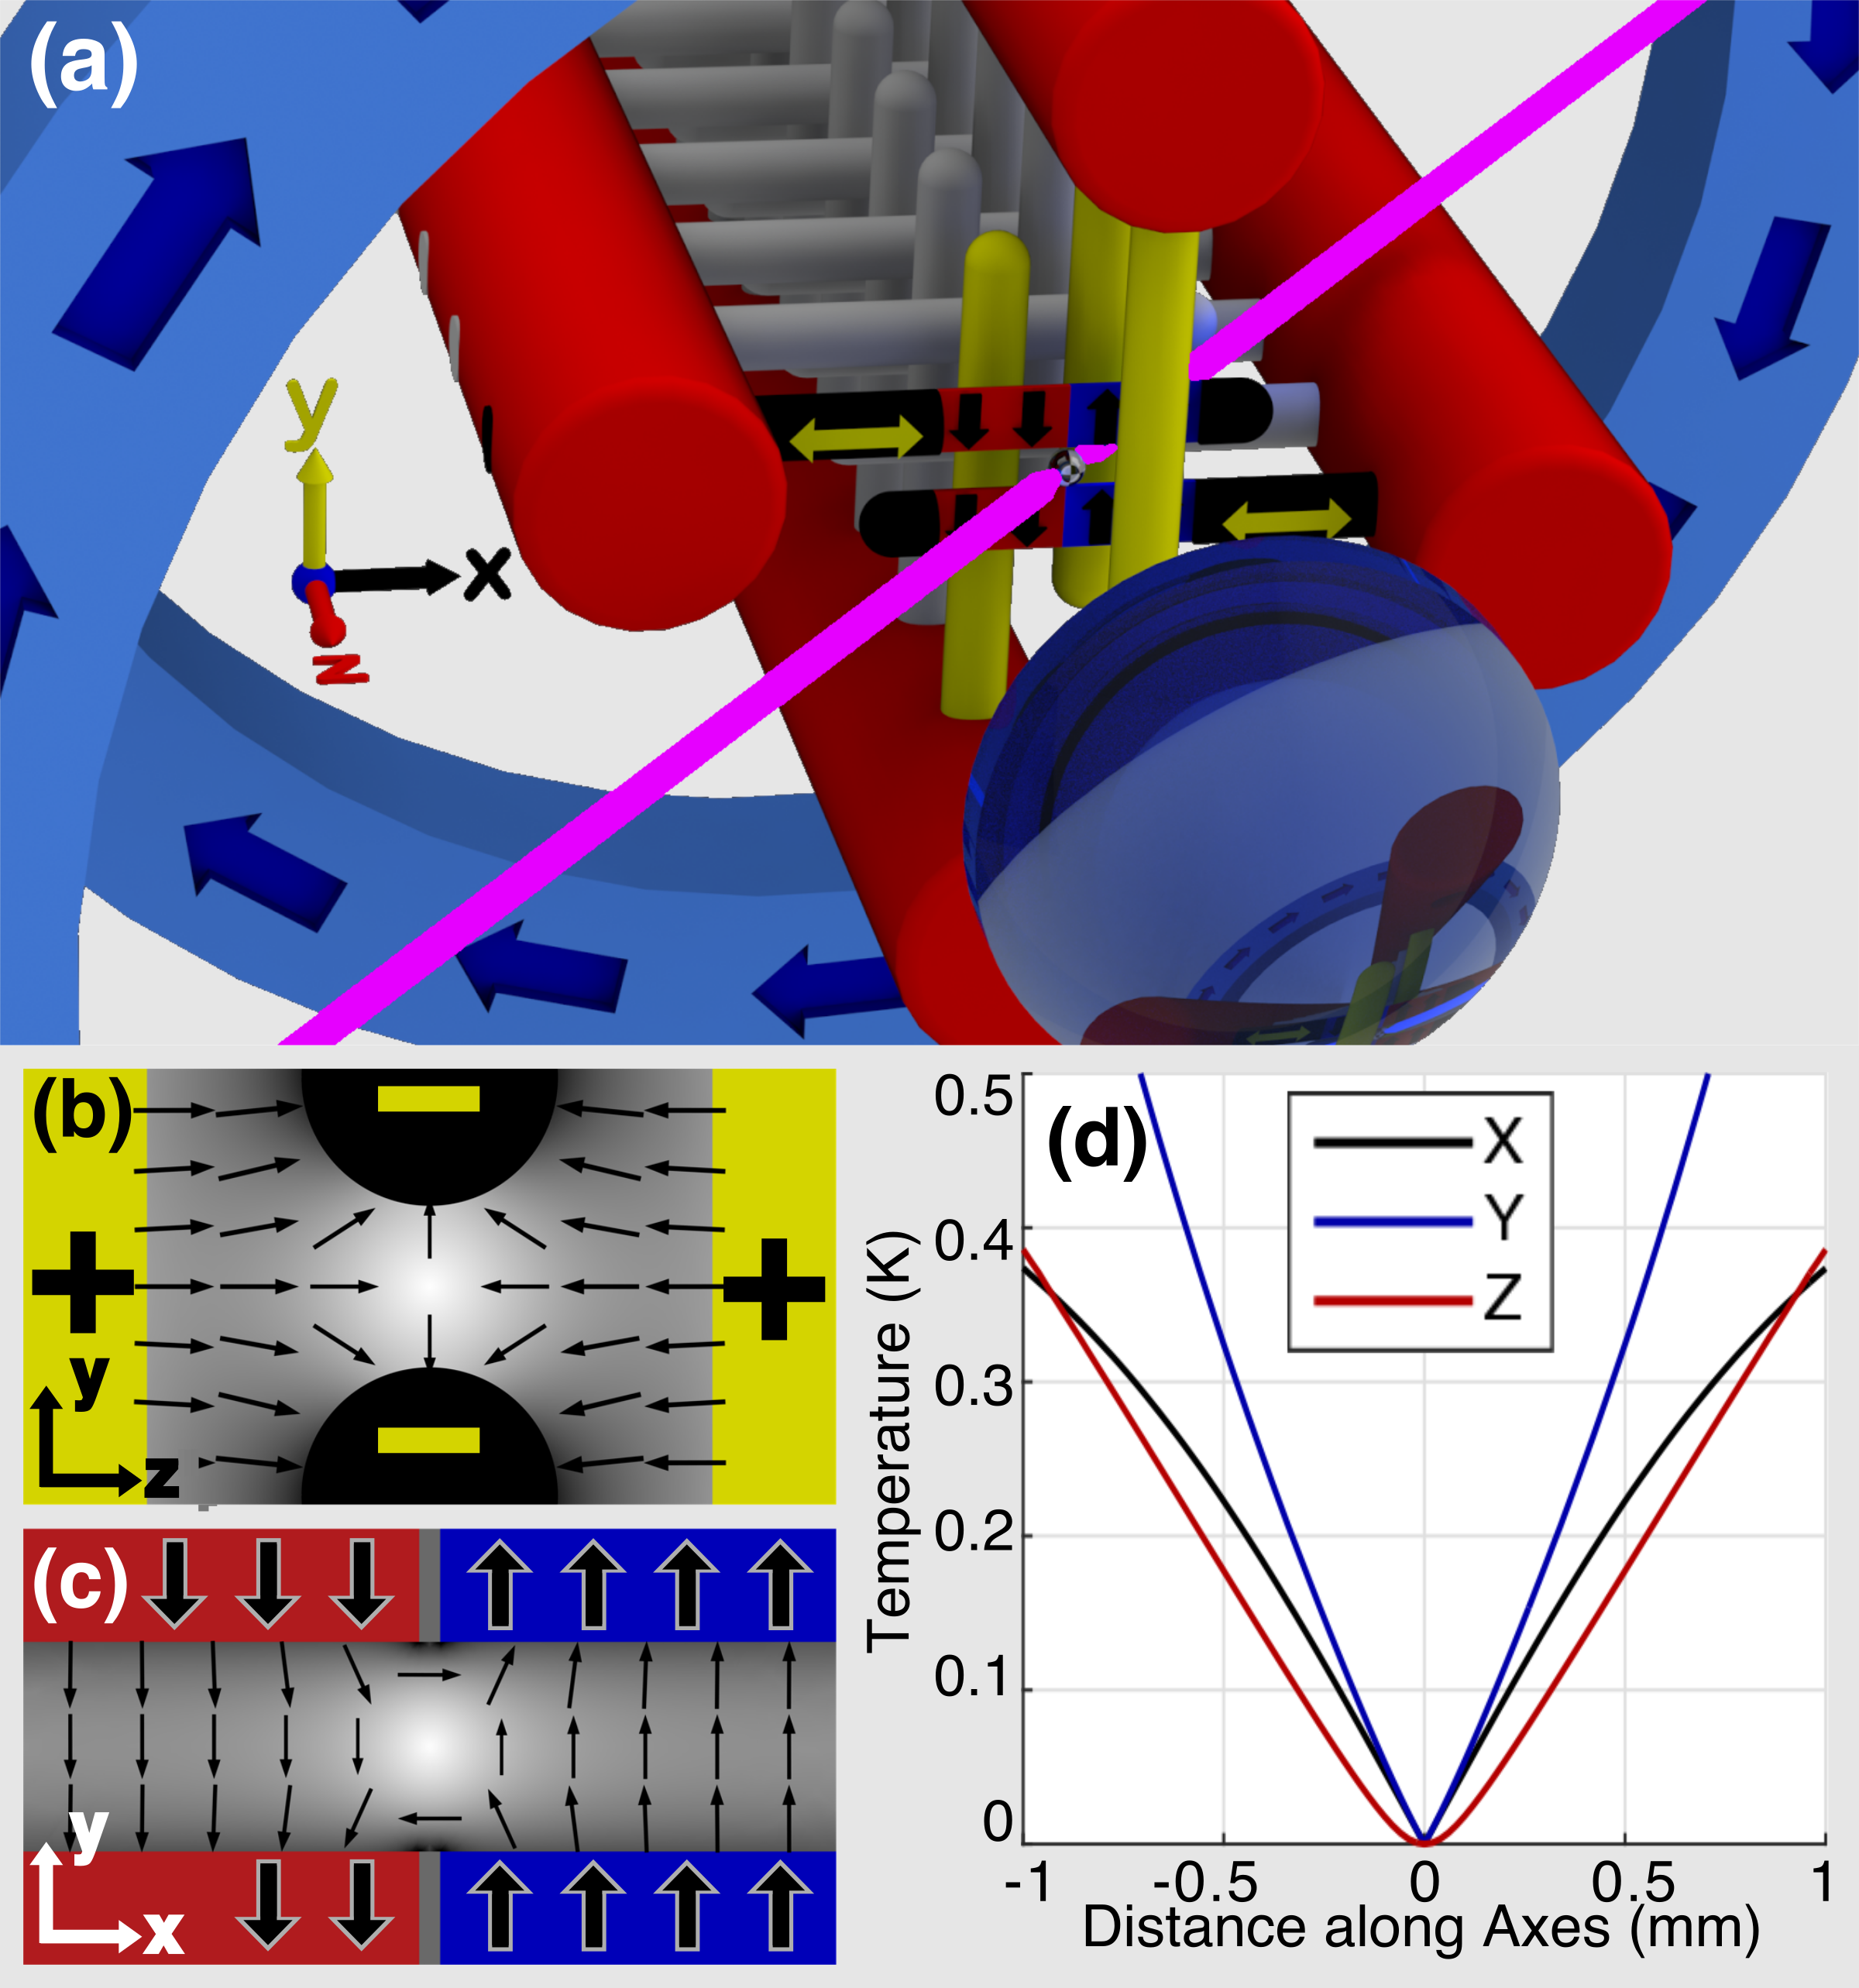
\includegraphics[width=\linewidth]{Geometry/CAD_recolor_laser_panels.PNG}%blue-red-yellow-v2_CAD.png}%
\caption{
Panel (a). Dual quadrupole trap embedded in Stark Decelerator. The decelerator has four backbone electrodes (red) and many pin electrodes (gray). OH produced and slowed as in~\cite{Sawyer2008}, except the slowing extends nearly to zero velocity between the second to last pin pair (black), magnetized as detailed in panel (c). Four pins then form the electric trapping quadrupole (yellow, one omitted for clarity), the last and third to last pin pairs. Detail in panel (b). Trapping pins are conductive with decelerator backbone; voltage configurations achieved with existing feedthroughs but modified MOSFET setup for bipolar output. Yellow bidirectional arrows indicate translations described in the text. Bias coils (light blue) and their current direction (dark blue) sit outside vacuum. LIF detection with laser (pink) and collection lens (blue). Panel (d) shows trap energy along axes. $B^\prime=5\text{ T/cm}$ and $E^\prime=100 \text{ kV/cm}^2$. Trap frequencies $\nu_x=3\text{ kHz}$, $\nu_y=5\text{ kHz}$, and $\nu_z=4\text{ kHz}$.\label{fig:CAD}}
\end{figure}
%Detection is realized via LIF with a $282\text{ nm}$ excitation in the x+y-z direction (pink) from $X^2\Pi_{3/2}(v=0)\rightarrow A^2\Sigma(v=1)$, and fluorescence at $313\text{ nm}$ from $A^2\Sigma(v=1)\rightarrow X^2\Pi_{3/2}(v=1)$ is focused by a lens (blue) onto a PMT in the z-direction.

We can sum up with a simple strategy: avoid $\mu_BB < d_EE$ where \epb. One way to obey this is to trap with E-field and superpose B-field. Although the lambda doublet prevents flips in this configuration, it also weakens the trap considerably, undesirable for maintaining large trap frequencies at low temperatures. Another option is to trap with both fields and keep zeros overlapped. This prevents spin-flip loss enhancement, but does not remove it entirely. It is also susceptible to misalignment induced spin-flip loss. A superposed magnetic quadrupole and electric hexapole has been realized for OH~\cite{Sawyer2007}. Although the use of only a single field would avoid spin-flip loss, any experiment which aims to make use of the doubly dipolar nature of molecules cannot accept this compromise.

Seeking to remove the loss entirely but without trap depth or trap gradient sacrifice, we use a pair of 2D quadrupole traps, one magnetic and the other electric, with orthogonal axes. We achieve these fields with a geometry that matches our Stark decelerator~\cite{Bochinski2003}, as shown in fig.~\ref{fig:CAD}. This approach is similar to the Ioffe-Pritchard strategy~\cite{pritchard1983}, where a 2D quadrupole is combined with an axial dipole trap. Axial and radial trapping interfere, resulting in significantly lower trap depths than the 3D quadrupole. We thwart this interference by using electric field for the third direction. This geometry has \epb along both the $x-z$ and $y-z$ planes, with $\mu_BB < d_EE$ in a large cylinder surrounding the $z$-axis. However, by adding magnetic field along the zero axis of the magnetic quadrupole with external bias coils, a fully tunable scenario emerges. %the \epb surface can be morphed into a hyperbolic sheet that does not approach closely to the magnetic minimum axis except far away from the trap center, thus preventing $\mu_BB < d_EE$.% , which can ``block" one another as discussed earlier but never result in an absolute decrease in potential energy of the doubly weak field seeking substate. 

%According to our intuition and our phase space coupling simulations, this integrated trap represents a near best-case scenario for coupling between a pulsed decelerator and a trap and ought to provide trap-averaged temperatures below $100\text{ mK}$. In practice we do not realize any significant molecule number increase relative to our previous trap geometries and temperatures are $170\text{ mK}$. This could be related to the difficulty of conditioning the magnet surfaces, which could be micro-discharging during operation leading to heating during loading. Finer polishing of the magnetic pins should address this.

\begin{figure}[tb]
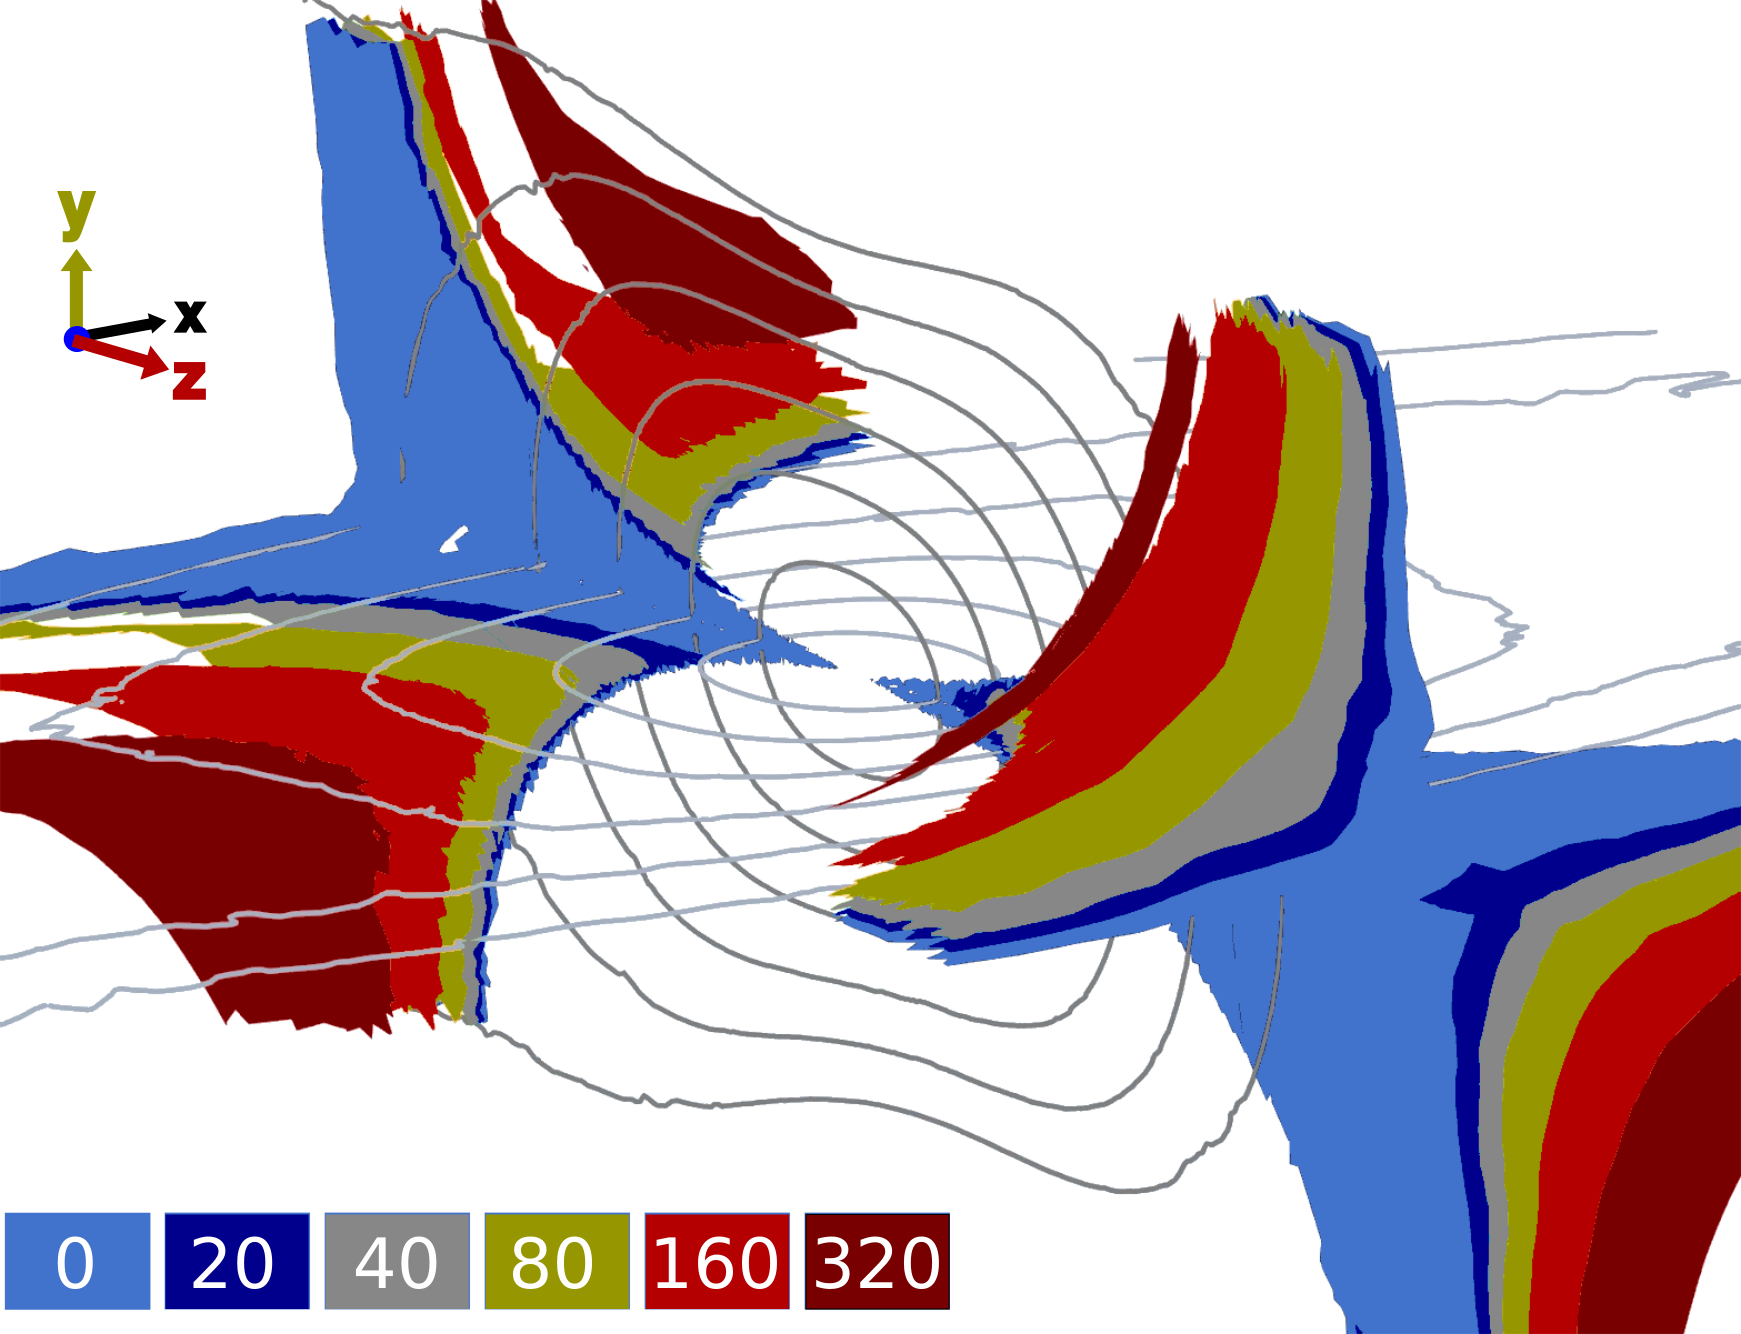
\includegraphics[width=\linewidth]{LossSurfaces/Loss_Surface_Chunks_recolored_legend.png}%
\caption{
Each color shows the surfaces where spin-flip can occur for the particular value of $B_\text{coil}$ given by the legend in units of Gauss. Trap energy contours are shown in gray. Larger $B_\text{coil}$ pushes the loss regions away from the trap center.
\label{fig:LSurfs}}
\end{figure}

$B_\text{coil}$ allows a full tuning from the fast $200\text{ s}^{-1}$ loss trace recorded in Panel (b) of Fig.~\ref{fig:WVplot} to complete removal. It does this by morphing the \epb surface from a pair of planes into a hyperbolic sheet which deviates spatially from the magnetic field minimum along the $z$-axis. Thanks to this deviation, for suitable magnitude of $B_\text{coil}$, $\mu_BB< d_EE$ can be avoided. In fig.~\ref{fig:LSurfs}, the surfaces where $B\!\perp\! E$ are colored wherever the splitting there is below the hopping threshold $\kappa$. Note how $B_\text{coil}$ tunes the proximity of the loss regions to zero. The loss regions are always visible, but they are tuned so far from the trap center that molecules accessing them have already escaped the trap.

\begin{figure}[tb]
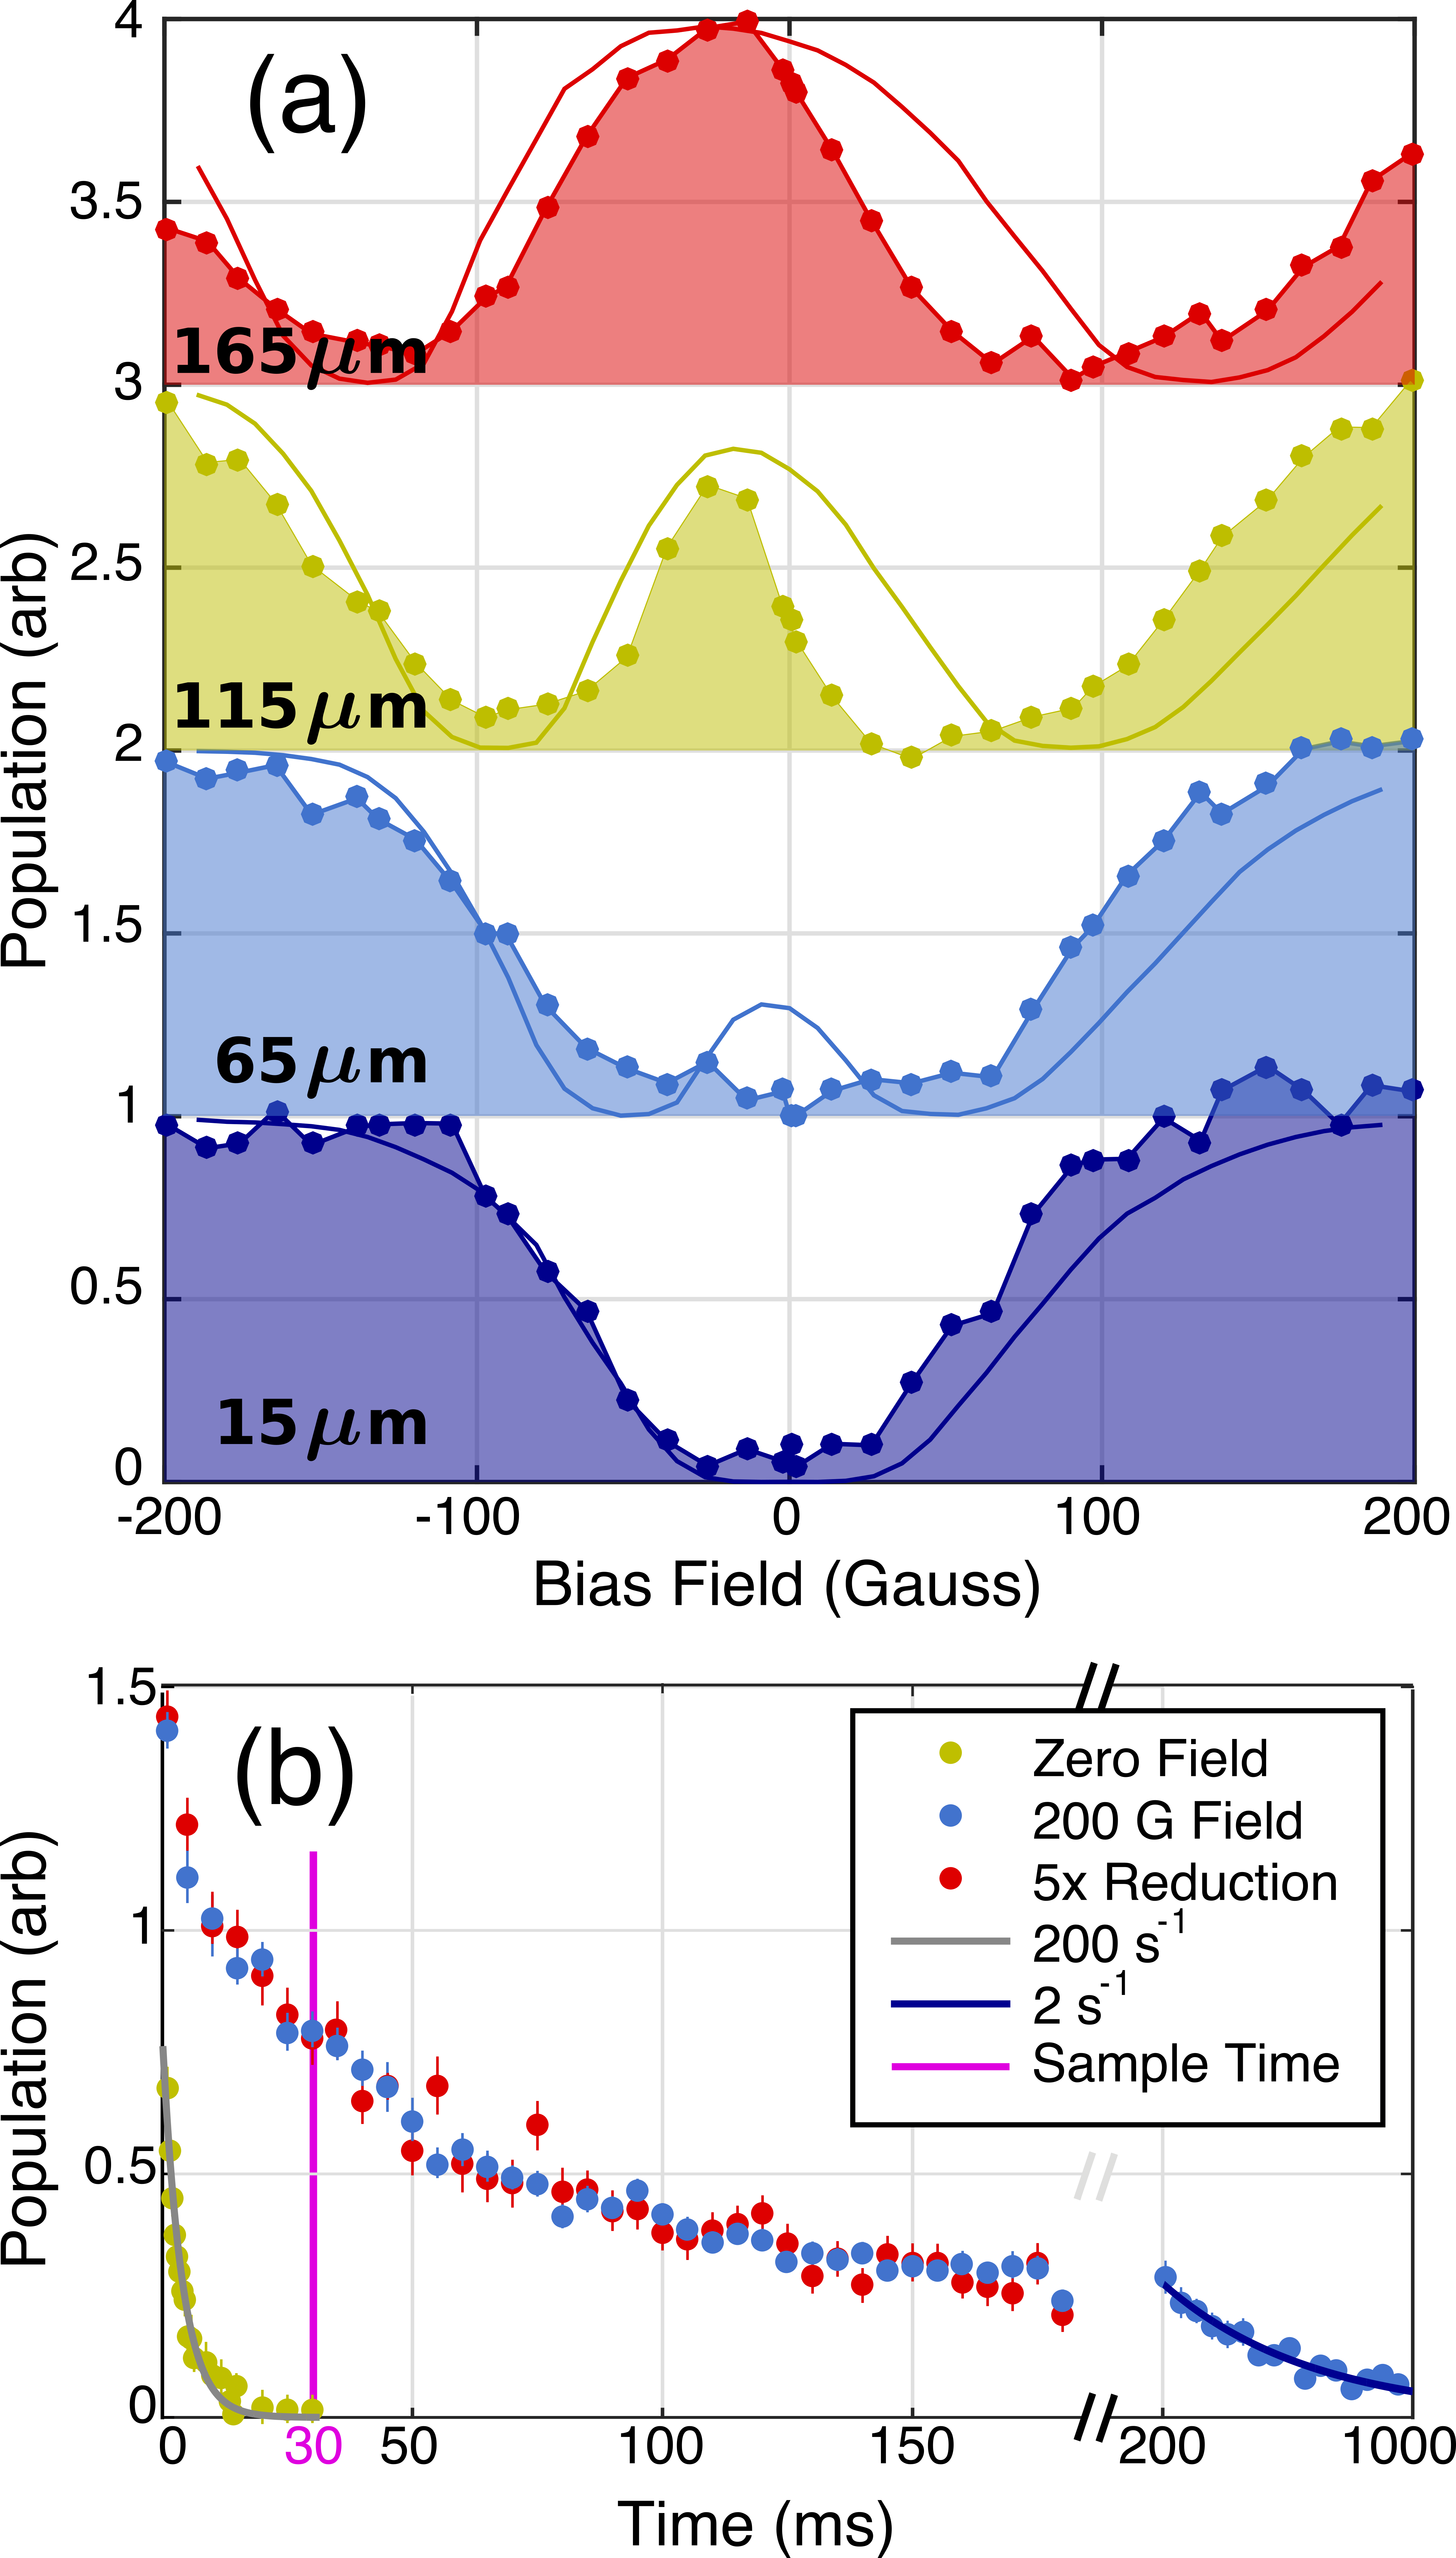
\includegraphics[width=\linewidth]{VWFig/tim-style-by-dave-1hz.png}%
\caption{
Panel (a). Family of curves showing the population after $30 \text{ms}$ as a function of pin translation and bias field. Panel (b). Time traces for aligned pins at two bias fields, a density modulated trace, and an extended time trace.
\label{fig:WVplot}}
\end{figure}

As a further confirmation of our \epb and $\mu_BB<d_EE$ model of the loss, we translate our magnetic pins in their mounts to alter the surface where \epb and compare experimental data against our expectations. The data are shown in fig.~\ref{fig:WVplot}. Qualitatively, this translation serves to disrupt the otherwise perfectly 2D magnetic quadrupole by adding a small trapping field $\vec{B}\propto B^\prime z\hat{z}$ along the z-axis. This means that $B_\text{coil}$ no longer directly tunes the minimum magnetic field in the trap. Instead, $B_\text{coil}$ must first overcome the slight trapping field along the $z$-axis, translating a point of zero field along the z axis and eventually out of the trap. The point of zero field disrupts the previously hyperbolic \epb surface, causing it to twist and intersect the $z$-axis near the magnetic zero. This intersection point has $\mu_BB<< d_EE$ except when aligned with the trap center, where $E$ also goes to zero. This means that without any bias field, the loss should actually be a local minimum; as the field is increased in either direction the loss should first worsen and then improve when the zero leaves the trap. This qualitative explanation correctly predicts the observed double well structure.

Quantitatively, we fit the family of curves shown in fig.~\ref{fig:WVplot} by performing an integration of molecule flux weighted by Landau-Zener probability and Maxwell-Boltzmann population density over the strangely twisted hyperbola of \epb. The computation is performed in COMSOL Multiphysics, accounting for the expected magnetic and electric fields from the trapping geometry with various offsets and with cloud temperature as the only free parameter.\footnote{Soure code is available: https://github.com/dreens/spin-flip-integration/}The fit temperature is approximately $170\text{ mK}$. The asymmetry of the curves about the $B_\text{coil}=0$ axis comes from a slight shift of the electric quadrupole minimum caused by an intentional bending of the last pin pair to increase fluorescence collection. This offset is not a free parameter in the model, it is directly included according to the measured bending applied to the pins. The fitted temperature is larger than expected from our simulations of the geometry, despite the known defocusing and reflection losses that accompany pulsed decelerators at low speeds~\cite{Sawyer2008a}. This may be related to micro-discharges on the surfaces of the magnetic pins during the final deceleration pulse. The magnetic pins are not currently polished as well as the rest of the decelerator, but this is not a fundamental limitation and could be overcome by diamond turning of the nickel plating on the pins or some other polishing strategy.

\begin{figure}[tb]
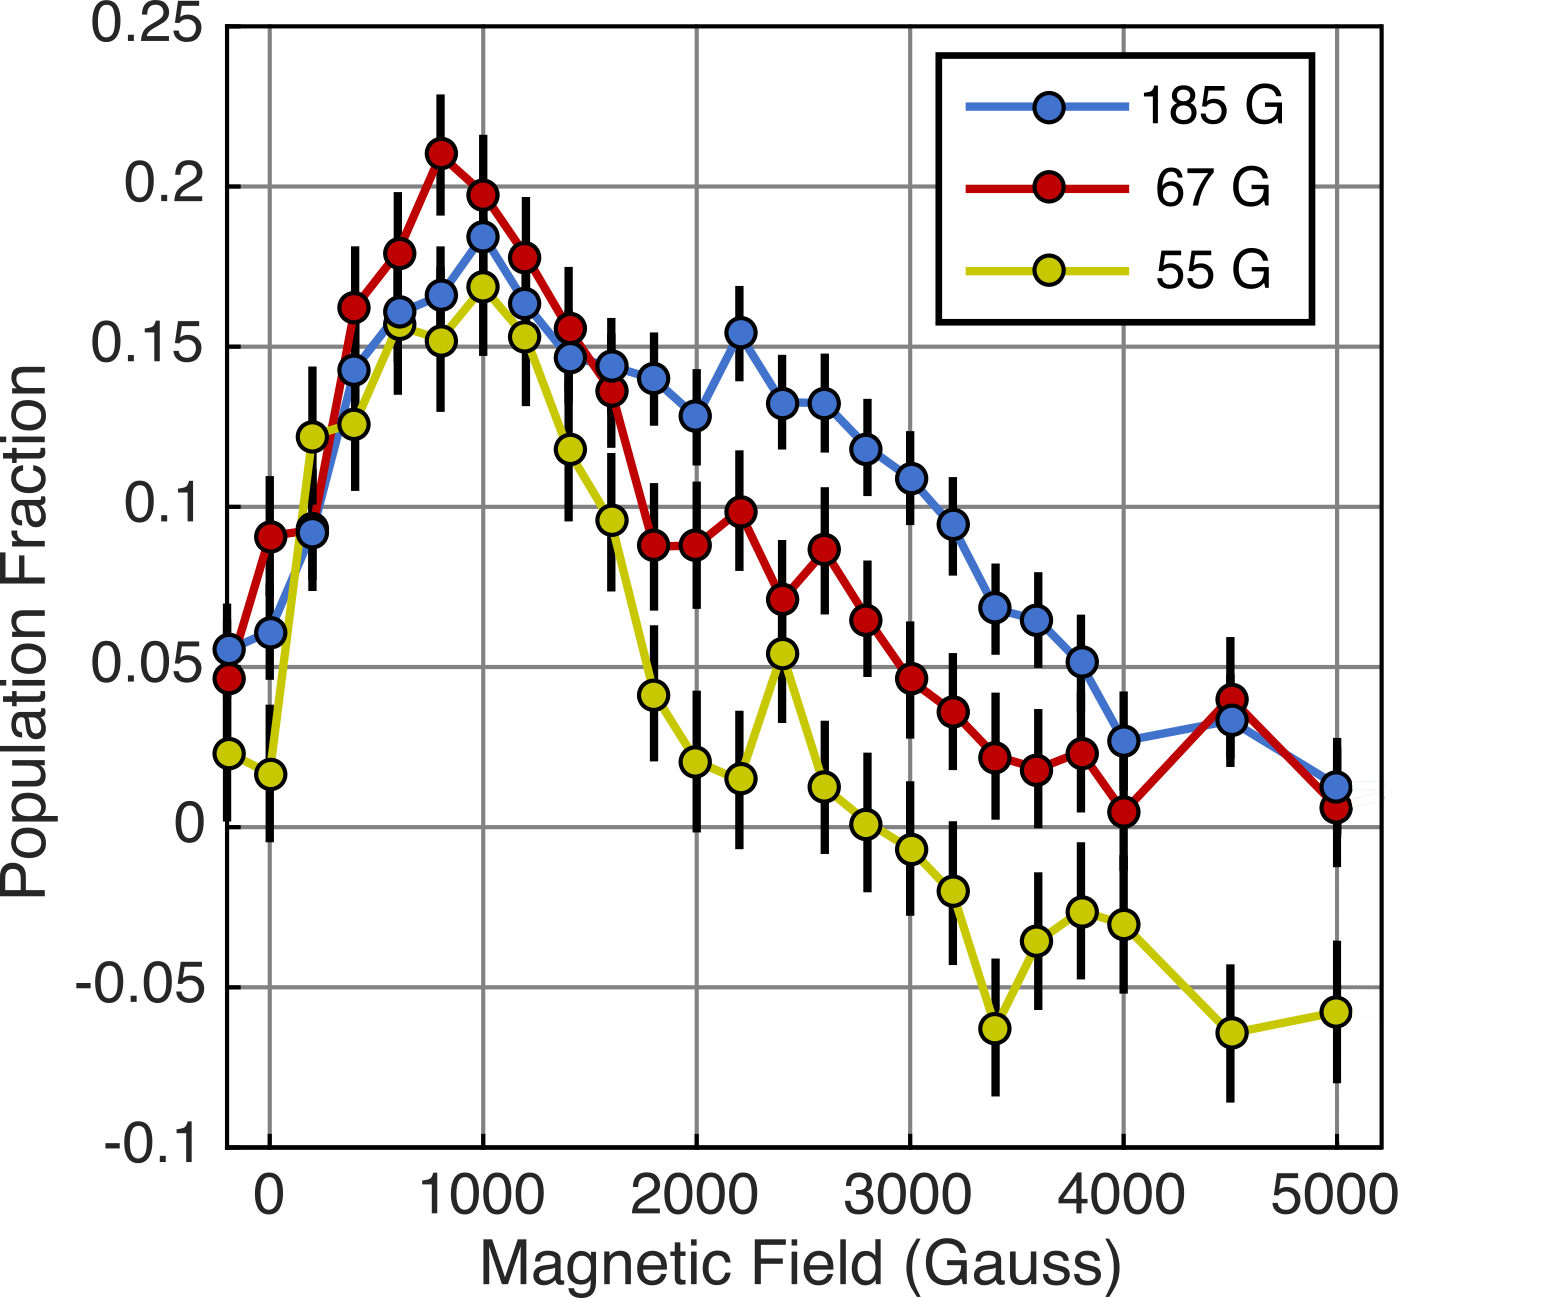
\includegraphics[width=\linewidth]{MWSpec/MW-therm-dave.png}%
\caption{
Microwave Thermometry. Bias field tunes the proximity of loss to the trap center. 
\label{fig:spec}}
\end{figure}

Another way to validate our understanding of molecular spin-flip loss in our dual quadrupole trap would be to confirm that the location of the loss is indeed tuned away from the trap center with increasing $B_\text{coil}$ as shown in fig.~\ref{fig:LSurfs}. We achieve this with a Zeeman microwave spectroscopy performed as in our previous work~\cite{Stuhl2012evap}. Rather than using a bias tee setup, a challenging prospect with our trap deeply integrated in the high voltage decelerator, we use a microwave probe to directly excite free space cavity modes of our vacuum chamber. The results are shown in fig.~\ref{fig:spec}. With the magnetic pins aligned, it is seen that higher values of $B_{\text{coil}}$ indeed increases the population of molecules able to survive at higher fields. In order to perform this spectroscopy, the trapping electric fields are switched off immediately prior to the application of a microwave transfer pulse tuned to a particular magnetic field strength. Thus the results reflect the Zeeman potential energy only, and only loosely correspond to the total potential energy of the molecules. Nonetheless, the shift in population center is clear and in agreement with our expectation.  %Roughly speaking, the average field of $2\text{ kG}$ corresponds to $200\text{ mK}$ for OH. Since this is approximately half the potential energy, we have $U\approx400\text{ mK}$. From the virial theorem for a linear trap, $U = 4.5k_BT$, so we can say the spectrum is consistent with $T\approx 90\text{ mK}$ and consistent with our fitting in fig.~\ref{fig:WVplot}.

In the case of lowest applied magnetic field in fig.~\ref{fig:spec}, i.e. deepest cutting of the loss region toward the trap center, a negative going signal is observed. This indicates a build-up in the opposite parity weak electric field seeking state. Although the spin-flips we have discussed connect strong and weak field seeking magnetic states, other avoided crossings amongst the ground state manifold result in the spin-flipped molecules remaining partially trapped in a secondary state with a nonuniform gradient (repulsive in the center, attractive outside) and a much lower overall trap depth. This secondary state also exhibits spin-flip loss to other lower states, but the enhancement with electric field is related to a quadratic blocking of the Zeeman splitting, and is thus not as dominating as the loss in the primary state due to cubic blocking.

Once the loss is fully removed, we observe the trend in blue on panel (b) of fig.~\ref{fig:WVplot}. The decay rate decreases with population over a timescale that is long compared with trap frequency and is thus suggestive of a collisional process. However, a completely phase-space blind density reduction technique \footnote{Microwaves applied via our free space cavity mode probe couple electrically weak and strong field seeking states during deceleration. The microwave wavelength of $15\text{ cm}$ is large compared with packet size, and the resonant energy corresponds to the low electric fields that all molecules experience when flying between stages.} that significantly reduces our molecule number causes little change in the shape of the trend, indicating that single-particle physics is responsible. This is attributable to our warmer initial temperature than in previous experiments. The slowly decaying trend could be related to the existence of high energy chaotic orbits with long escape times, as seen in other exotically shaped trapping potentials~\cite{Gonzalez-Ferez2014}. We hope in the near future to implement an increase in molecule number rather than a decrease, by means of a suite of density enhancing experimental improvements.

Our dual quadrupole trap decisively overcomes molecule enhanced spin-flip loss by tuning it from an overwhelming rate to complete removal. Our explanation of the loss provides detailed predictions of how its location and magnitude ought to scale with bias field and trap alignment, which we have experimentally verified. Our results contradict existing predictions about molecular spin-flips in mixed fields and we provide a consistent framework that explains this based on internal spin-dynamics. We have devised a viable trapping geometry in which spin-flip loss is fully mitigated without trap-depth sacrifice, paving the way toward further improvements in molecule trapping and cooling.

We acknowledge our the Gordon and Betty Moore Foundation and the AFOSR for their financial support. T.L. acknowledges support by the Alexander von Humboldt Foundation through a Feodor Lynen Fellowship. We thank J.L. Bohn and S.Y.T. van de Meerakker for helpful discussions.

D.R. and H.W. contributed equally to this work: D.R. in writing and trap design, H.W. in experiment execution.

%includes uncited bib entries
%\nocite{*}
\bibliographystyle{apsrev4-1_no_Arxiv}
\bibliography{MolecularMajoranaLoss}% Produces the bibliography via BibTeX.

\end{document}
%
% ****** End of file MolecularMajoranaLoss.tex ******
